% !TeX encoding = UTF-8
\documentclass[aspectratio=169]{beamer}
\useoutertheme[progressbar=frametitle]{metropolis}
\useinnertheme{metropolis}
\definecolor{nabgray}{rgb}{0.6,0.59,0.61}
\usecolortheme[named=nabgray]{structure}

\usepackage{tikz}
\usepackage[utf8]{inputenc}
\usepackage[spanish]{babel}
\usepackage{fontspec}
\setmonofont{JetBrains Mono}
\setmainfont{Roboto}
\setsansfont{Roboto}

\usepackage{smartdiagram}
\usepackage{qtree}
\usepackage{verbatim}
\usepackage{svg}
\usepackage{graphicx}
\usepackage{color}

\definecolor{lightgray}{rgb}{0.95, 0.95, 0.95}
\definecolor{darkgray}{rgb}{0.4, 0.4, 0.4}
%\definecolor{purple}{rgb}{0.65, 0.12, 0.82}
\definecolor{editorGray}{rgb}{0.95, 0.95, 0.95}
\definecolor{editorOcher}{rgb}{1, 0.5, 0} % #FF7F00 -> rgb(239, 169, 0)
\definecolor{editorGreen}{rgb}{0, 0.5, 0} % #007C00 -> rgb(0, 124, 0)
\definecolor{orange}{rgb}{1,0.45,0.13}
\definecolor{olive}{rgb}{0.17,0.59,0.20}
\definecolor{brown}{rgb}{0.69,0.31,0.31}
\definecolor{purple}{rgb}{0.38,0.18,0.81}
\definecolor{lightblue}{rgb}{0.1,0.57,0.7}
\definecolor{lightred}{rgb}{1,0.4,0.5}
\usepackage{upquote}
\usepackage{listings}
\lstset{language=java,
	basicstyle=\footnotesize\ttfamily,
	keywordstyle=\footnotesize\color{blue}\ttfamily,
	escapeinside={<@}{@>}
}


\usebackgroundtemplate%
{%
	
\includegraphics[width=\paperwidth]{Images/Contenido}%
}


\title{Desarrollo moderno con DevOps y Cloud Native}
\author{Víctor Orozco}
\institute{Nabenik}
\date{\today}

\begin{document}





{
    \usebackgroundtemplate{
\includegraphics[width=\paperwidth]{Images/portada}}
    \setbeamercolor{frametitle}{fg=red}
    \usebeamercolor[fg]{normal text}
    \frame{\titlepage}
}


\begin{frame}{Aplicaciones reactivas}

\begin{figure}
	\centering
	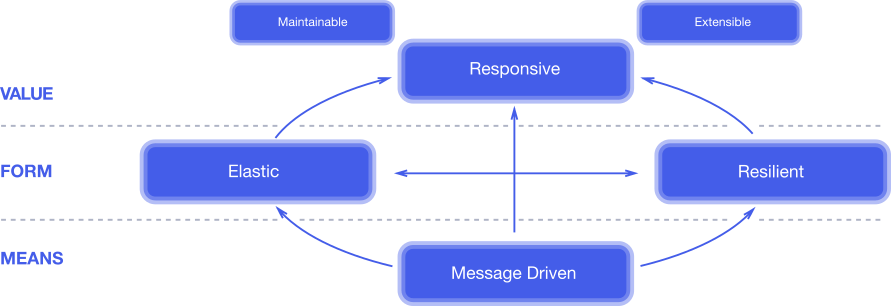
\includegraphics[width=\linewidth]{Images/reactive-traits.png}
\end{figure}

\end{frame}




\begin{frame}{Cloud native}

	\begin{itemize}
		\item Sistemas reactivos
		\item 12 factores cloud native
        \item Design patterns
        \item Domain Driven Design
		\item Microservices chassis e/ou service mesh
        \item Orquestación de contenedores
	\end{itemize}

\end{frame}


\begin{frame}{Cloud native}

	\begin{itemize}
		\item (Nos gustaria tener) Sistemas reactivos
		\item (Es posible con la metodología de) 12 factores Cloud Native
        \item (Usamos soluciones probadas mediante) design patterns
        \item (Fragmentamos el sistema mediante) Domain Driven Design
		\item (Implementamos los servicios con) Microservices chassis y/o service mesh
        \item (Hacemos deployment) Mediante orquestación de containers
	\end{itemize}


\end{frame}


\begin{frame}{Historia}

\begin{figure}
	\centering
	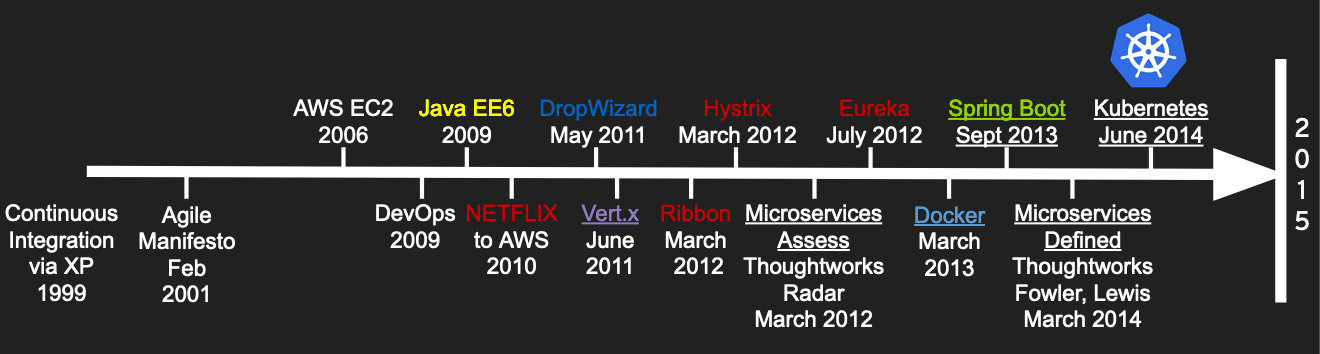
\includegraphics[width=\linewidth]{Images/timeline}
\end{figure}
Créditos: Rafael Benevides

\end{frame}



{
    \usebackgroundtemplate{
\includegraphics[width=\paperwidth]{Images/separador}}
    \setbeamercolor{normal text}{fg=white}
    \setbeamercolor{frametitle}{fg=red}
    \usebeamercolor[fg]{normal text}
    \section{12 factores Cloud Native}
}


\begin{frame}{12 factores cloud native (Heroku)}

\begin{columns}[T] % contents are top vertically aligned

	\begin{column}[T]{4cm} % alternative top-align that's better for graphics
		\begin{alertblock}{Frameworks}
			\begin{itemize}
				\item Config
				\item Backing service
				\item Disposability
			\end{itemize}
		\end{alertblock}
	\end{column}
	\begin{column}[T]{6cm} % each column can also be its own environment
		\begin{block}{Cloud}
			\begin{itemize}
				\item Codebase (Git-Flow)
				\item Dependencies (Maven)
				\item Build, Release, Run
				\item Processes
				\item Port binding
				\item Concurrency (Docker - k8s)
				\item Dev / Prod parity
				\item Logs
				\item Admin process
			\end{itemize}
		\end{block}
	\end{column}
\end{columns}

\end{frame}

\begin{frame}{Codebase}
\begin{itemize}
	\item Una base de código con múltiples entornos de despliegue
	\item Un repositorio por aplicación / microservicio
\end{itemize}

\begin{figure}
	\centering
	
\includegraphics[width=0.5\linewidth]{Images/121}
\end{figure}
\end{frame}


\begin{frame}{Dependencias}
\begin{itemize}
	\item Una aplicación cloud native no "depende" de algo en su entorno
	\item Dependencias isoladas y compilaciones repetibles
\end{itemize}

\begin{figure}
	\centering
	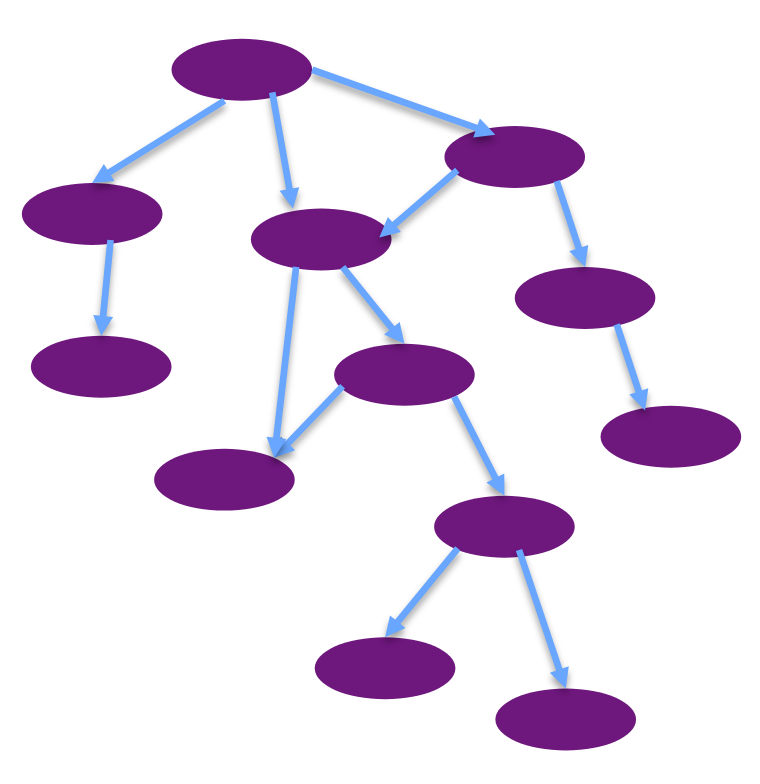
\includegraphics[width=0.4\linewidth]{Images/maven}
\end{figure}
\end{frame}


\begin{frame}{Configuración}
\begin{itemize}
	\item La configuración de una aplicación debe ser dinámica sin re-compilación/re-empaque
	\item Configuraciones inyectables
\end{itemize}
\end{frame}


\begin{frame}{Backing services}
\begin{itemize}
	\item Acoplamiento debil. Siempre tratar backing services como componentes intercambiables y/o adjuntos
\end{itemize}

\begin{figure}
	\centering
	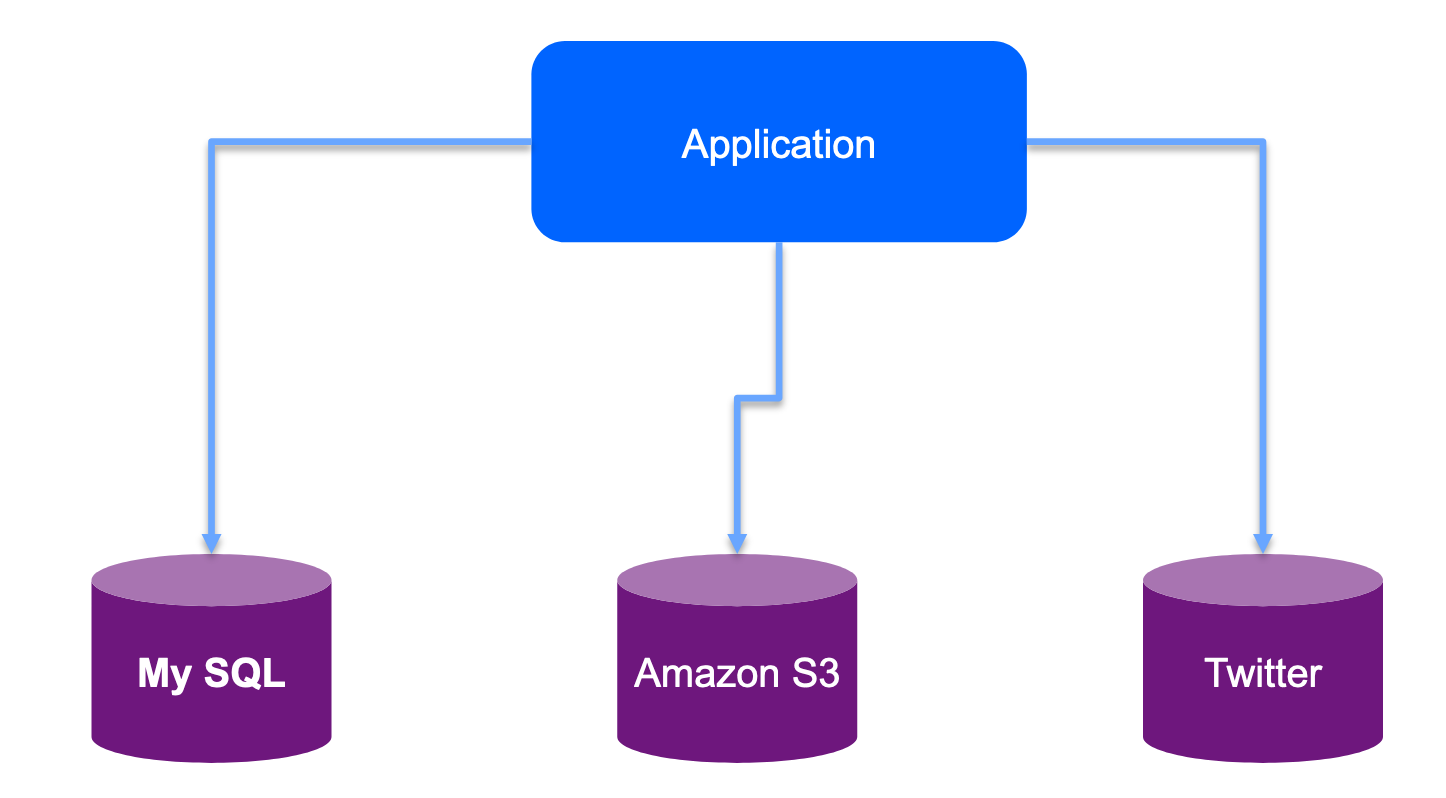
\includegraphics[width=0.5\linewidth]{Images/backing}
\end{figure}
\end{frame}

\begin{frame}{Build, release, run}
\begin{itemize}
	\item Separación de etapas de construcción, ejecución y lanzamiento
	\item CI/CD se hace obligatorio
\end{itemize}
\end{frame}

\begin{frame}{Procesos}
\begin{itemize}
	\item Ejecutar la aplicación como uno o más procesos sin estado
	\item REST, Stateless, sesiones portables con JWT
\end{itemize}
\begin{figure}
	\centering
	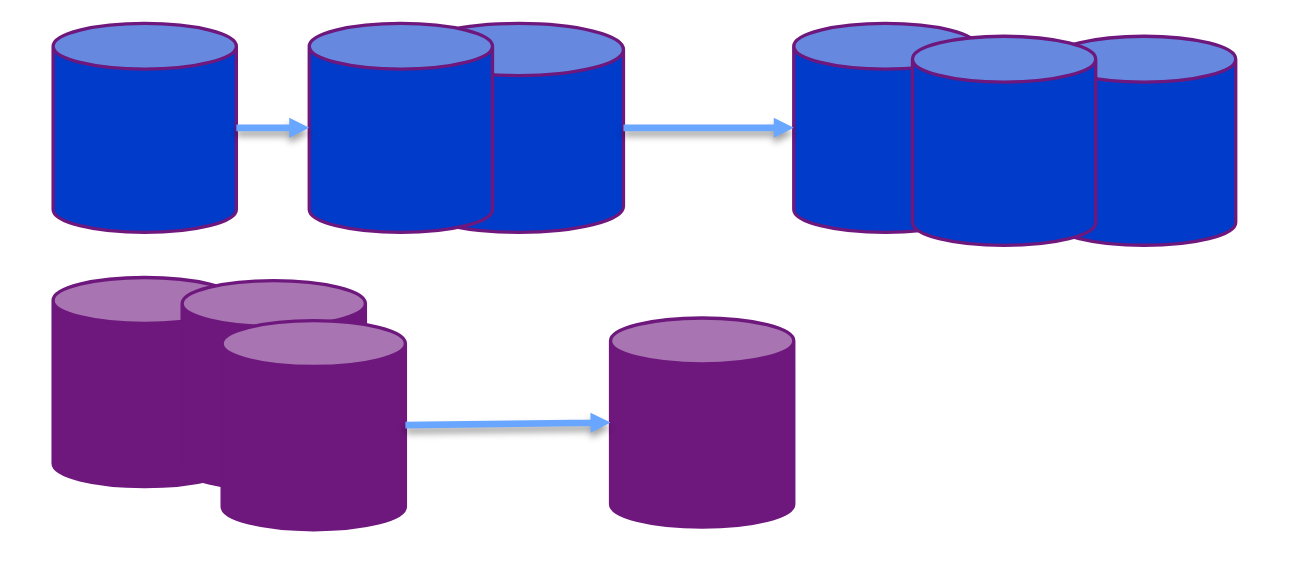
\includegraphics[width=0.5\linewidth]{Images/services}
\end{figure}
\end{frame}


\begin{frame}{Port binding}
\begin{itemize}
	\item Exponer los servicios con puertos dinámicos
	\item Kubernetes, Docker, etc.
\end{itemize}
\end{frame}

\begin{frame}{Concurrencia}
\begin{itemize}
	\item Aplicaciones escalan de forma independiente replicándose
	\item Las nubes escalan mediante copias independientes, sin estado
\end{itemize}
\end{frame}

\begin{frame}{Disposability}
\begin{itemize}
	\item Procesos arrancar rápido, mueren rápido, reinician rápido
	\item Procesos son tolerantes a fallas
\end{itemize}

\end{frame}

\begin{frame}{Dev/Prod parity}
\begin{itemize}
	\item Entornos de desarrollo, certificación, producción lo más homogéneos posible
\end{itemize}
\end{frame}

\begin{frame}{Logs}
\begin{itemize}
	\item Manipular logs de n copias de n servicios (streams de eventos)
	\item Permitir el análisis posterior
\end{itemize}
\end{frame}

\begin{frame}{Admin process}
\begin{itemize}
	\item Manipular logs de n copias de n servicios (streams de eventos)
	\item Permitir el análisis posterior
\end{itemize}
\end{frame}
{
    \usebackgroundtemplate{
\includegraphics[width=\paperwidth]{Images/separador}}
    \setbeamercolor{normal text}{fg=white}
    \setbeamercolor{frametitle}{fg=red}
    \usebeamercolor[fg]{normal text}
    \section{Estrategia}
}

\begin{frame}{Estrategia}
\begin{itemize}
	\item Implementar DevOps sobre la base de código actual
    \item Evaluar opciones Cloud Native completas
    \item Fragmentar en Microservicios solo si es necesario
\end{itemize}
\end{frame}

{
    \usebackgroundtemplate{
\includegraphics[width=\paperwidth]{Images/separador}}
    \setbeamercolor{normal text}{fg=white}
    \setbeamercolor{frametitle}{fg=red}
    \usebeamercolor[fg]{normal text}
    \section{DevOps}
}

\begin{frame}{Etapas}
\begin{figure}
	\centering
	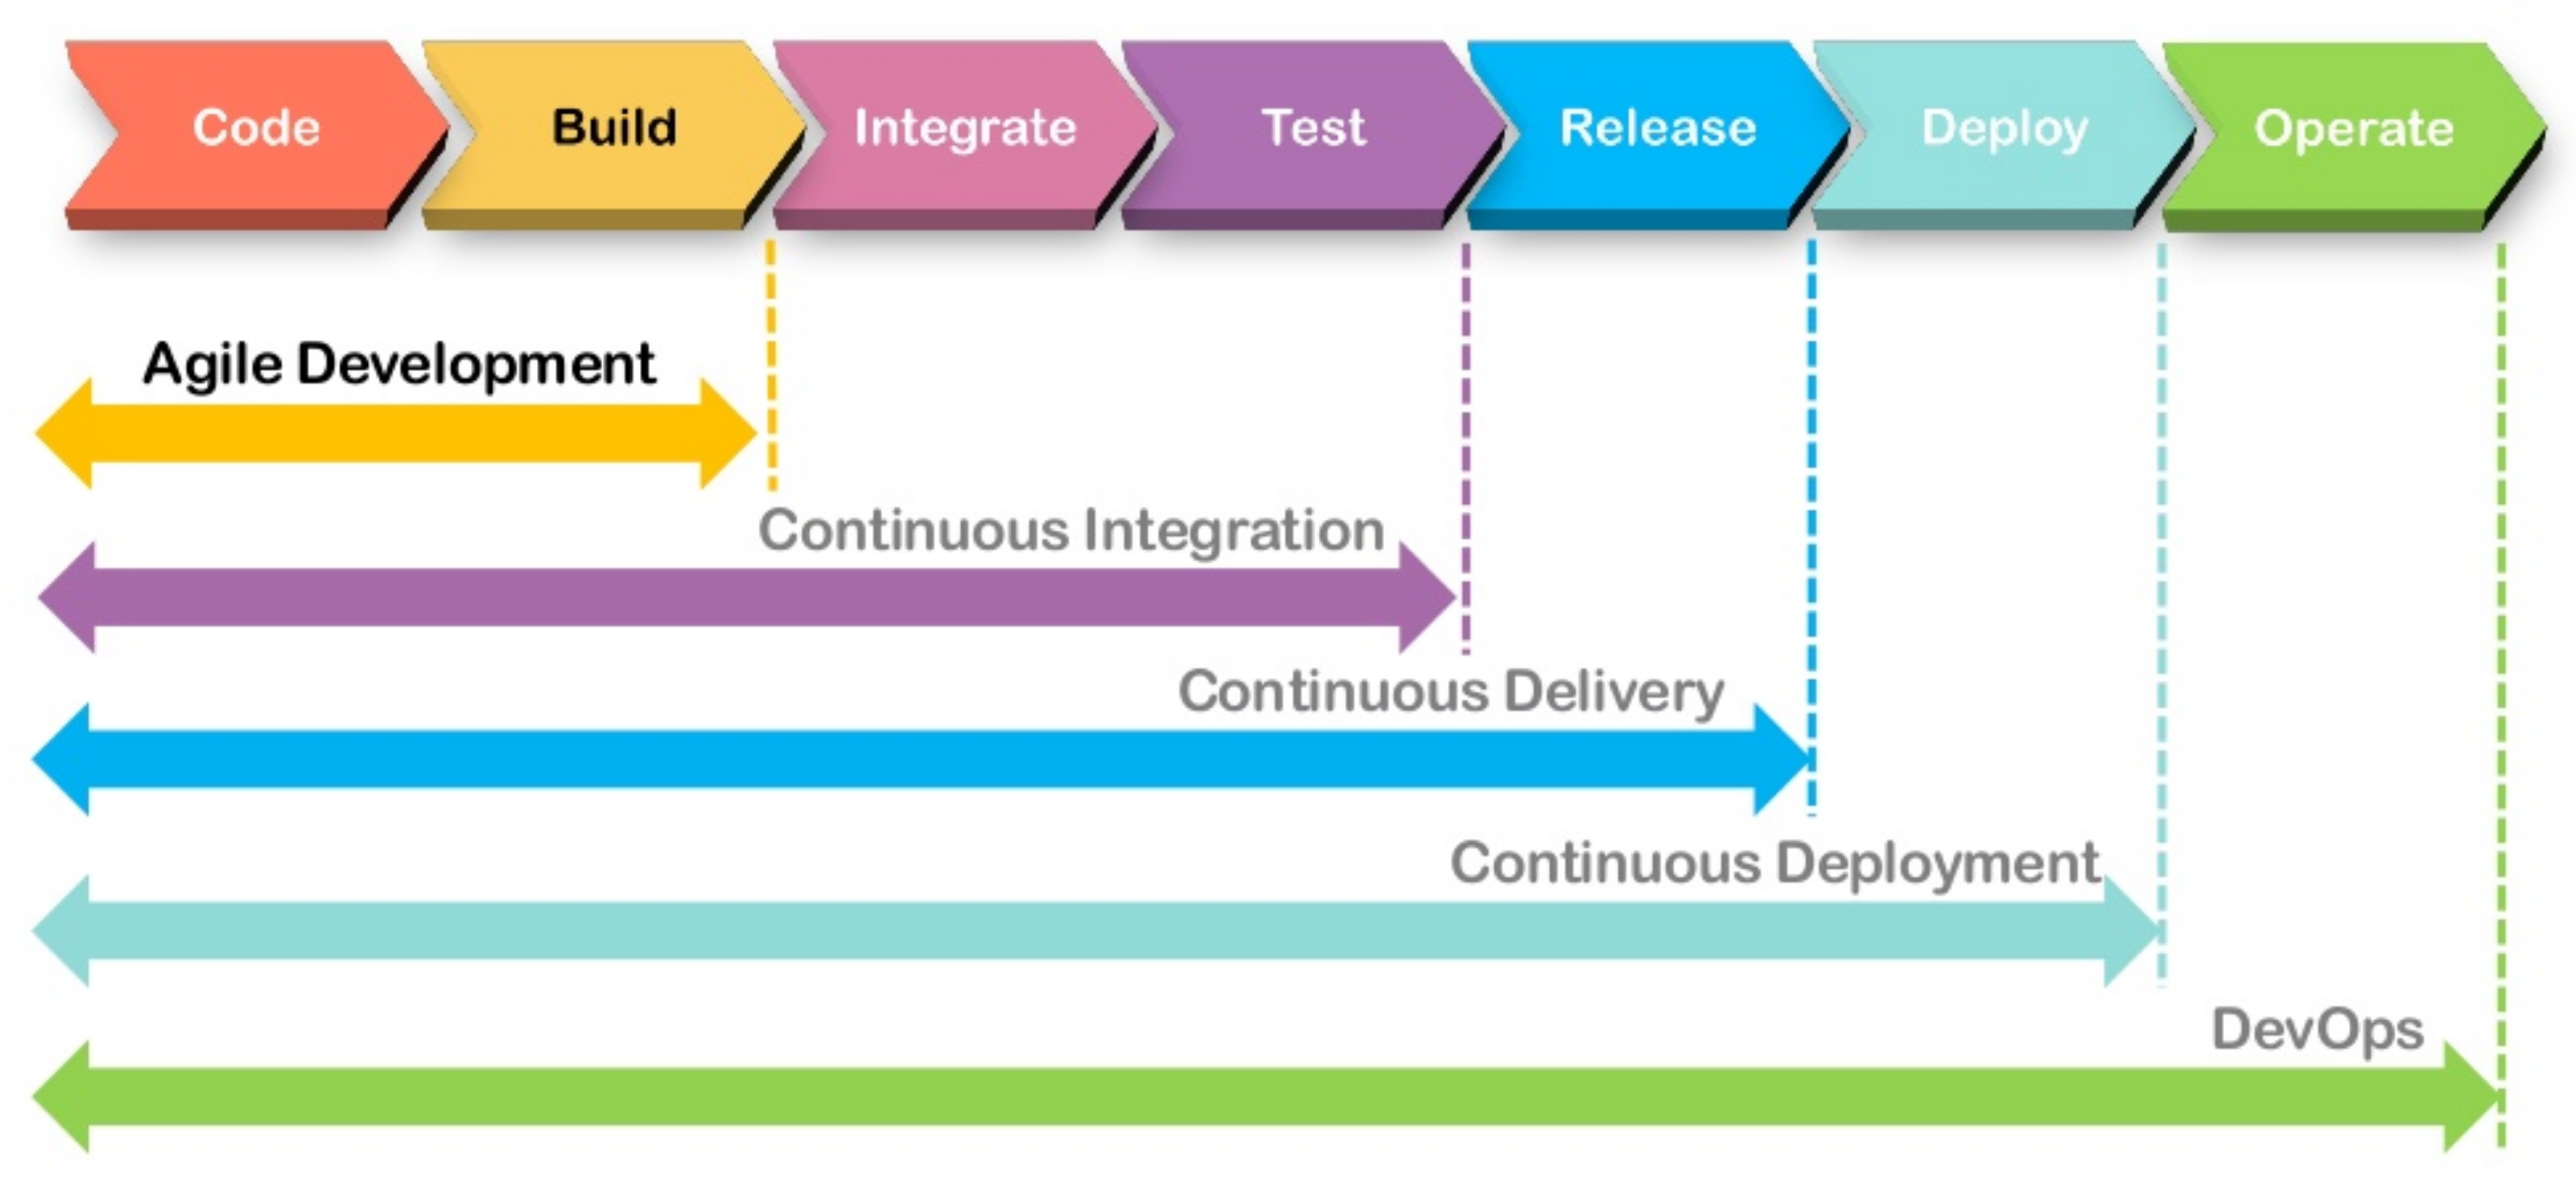
\includegraphics[width=\linewidth]{Images/etapa1}
	\label{fig:etapa1}
\end{figure}
\end{frame}

\begin{frame}{Delivery vs Deployment}
\begin{figure}
	\centering
	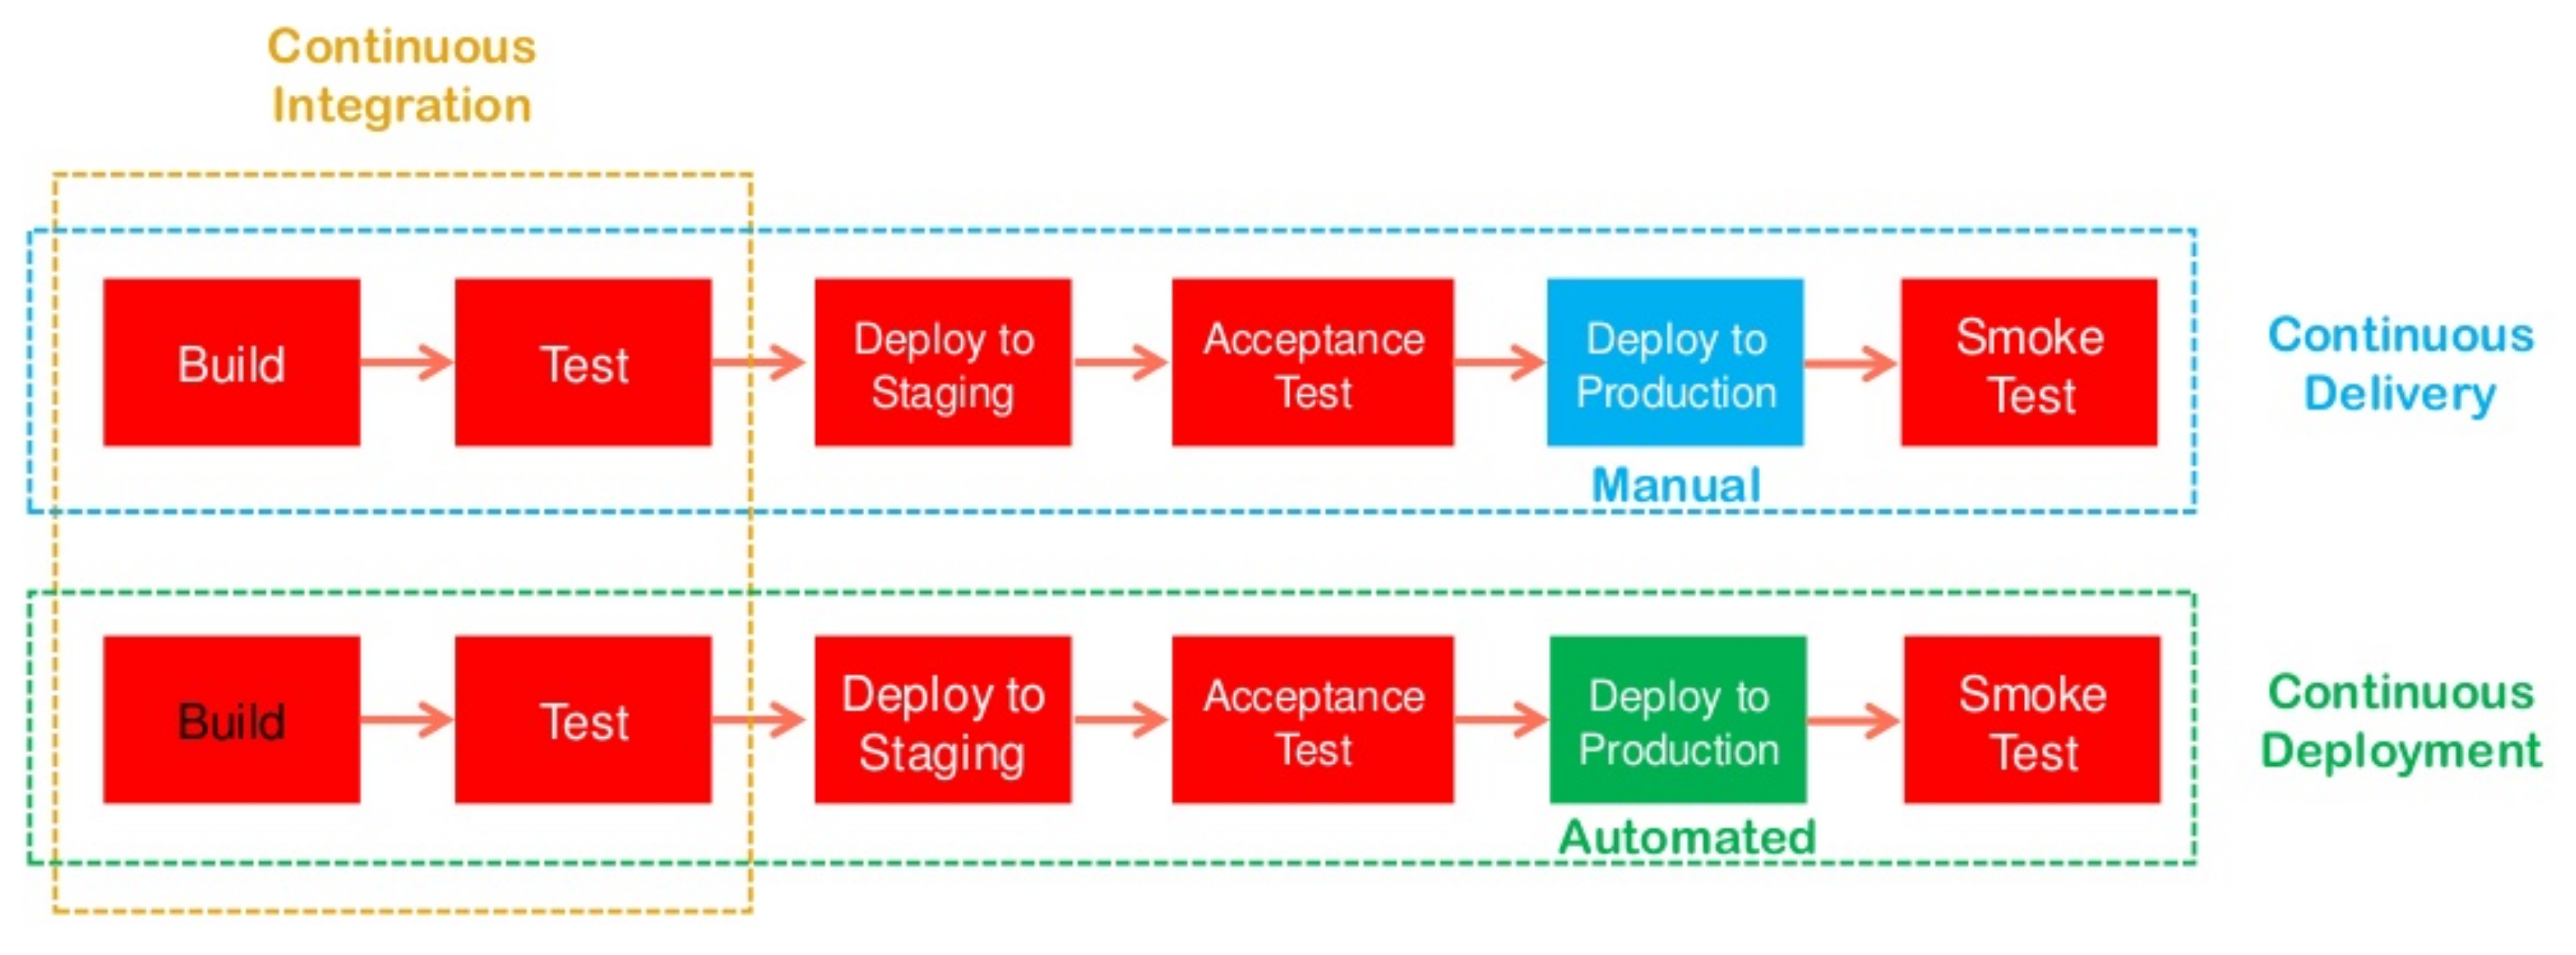
\includegraphics[width=\linewidth]{Images/etapa2}
	\label{fig:etapa2}
\end{figure}
\end{frame}

{
    \usebackgroundtemplate{
\includegraphics[width=\paperwidth]{Images/separador}}
    \setbeamercolor{normal text}{fg=white}
    \setbeamercolor{frametitle}{fg=red}
    \usebeamercolor[fg]{normal text}
    \section{Patrones nuevos}
}



\begin{frame}{}
\begin{figure}
	\centering
	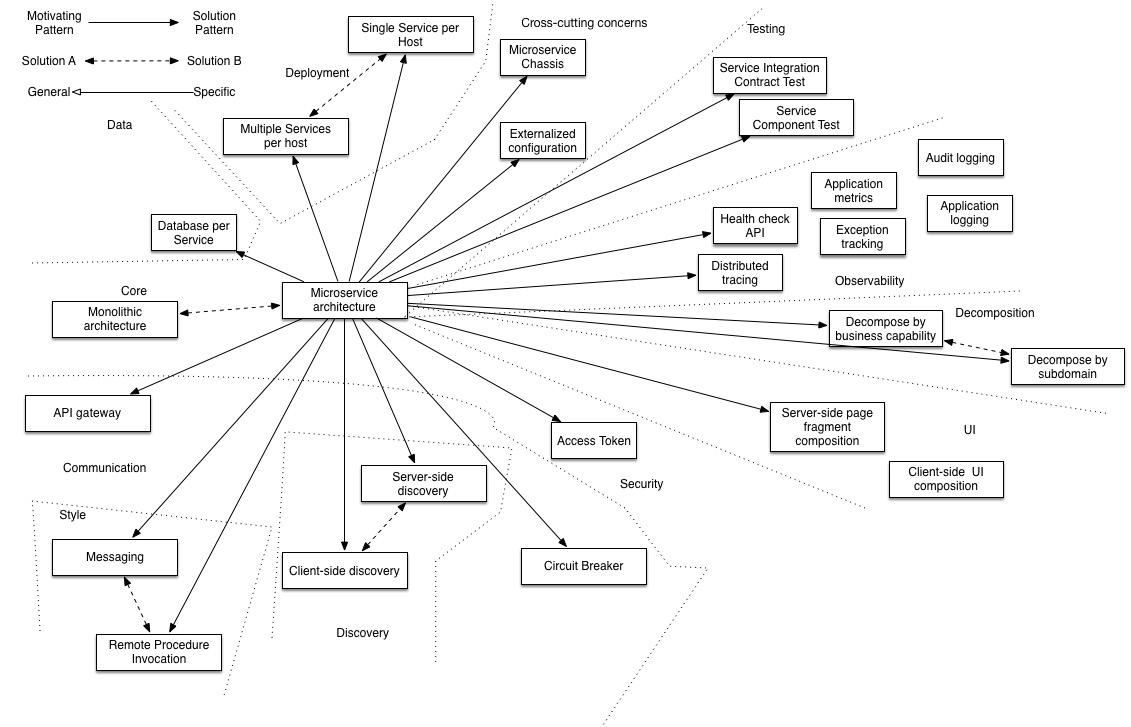
\includegraphics[width=\linewidth]{Images/PatternsRelatedToMicroservices}
\end{figure}
\end{frame}

\begin{frame}{}
\begin{figure}
	\centering
	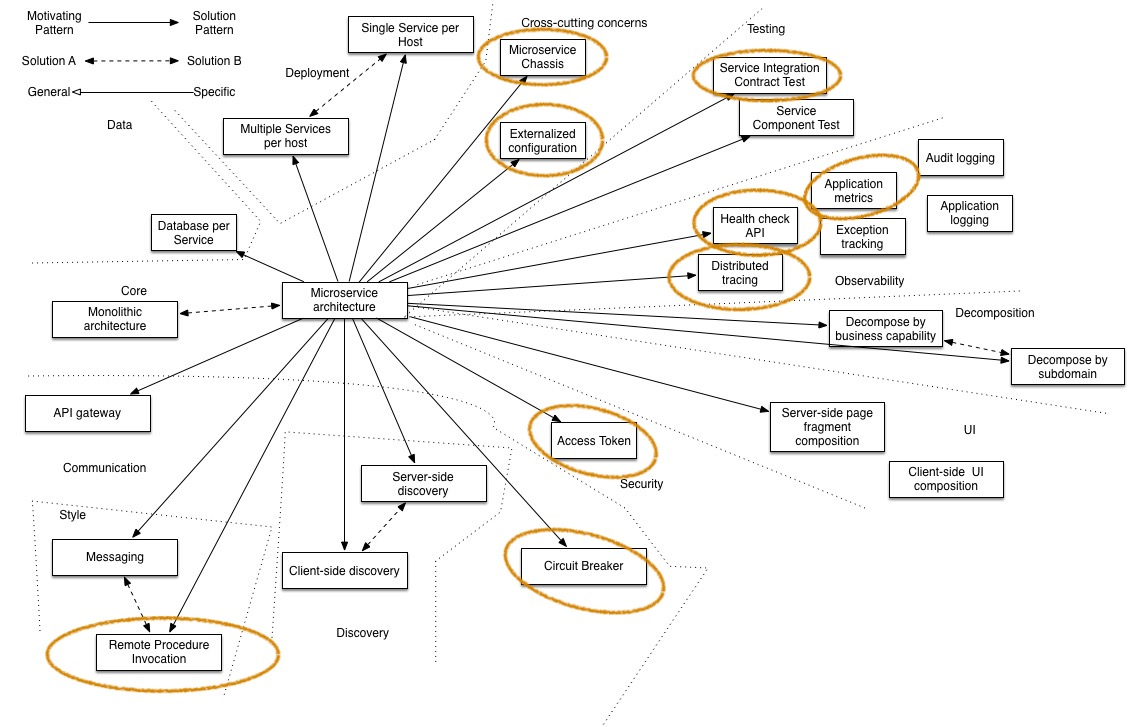
\includegraphics[width=\linewidth]{Images/PatternsRelatedToMicroservices2}
\end{figure}
\end{frame}



{
    \usebackgroundtemplate{
\includegraphics[width=\paperwidth]{Images/separador}}
    \setbeamercolor{normal text}{fg=white}
    \setbeamercolor{frametitle}{fg=red}
    \usebeamercolor[fg]{normal text}
    \section{Microservice Chassis}
}

\begin{frame}{Microservice Chassis}



\begin{columns}[T] % contents are top vertically aligned
\begin{column}[T]{6cm} % each column can also be its own environment
	\begin{block}{Chassis}
    Los frameworks Cloud Native son soluciones para problemas "cross-cuting concerns".
	\end{block}
    \begin{block}{Chassis Java}
Spring Boot, MicroProfile, DropWizard, Akka
	\end{block}
\end{column}
\begin{column}[T]{7cm} % alternative top-align that's better for graphics
    \begin{figure}
    	\centering
    	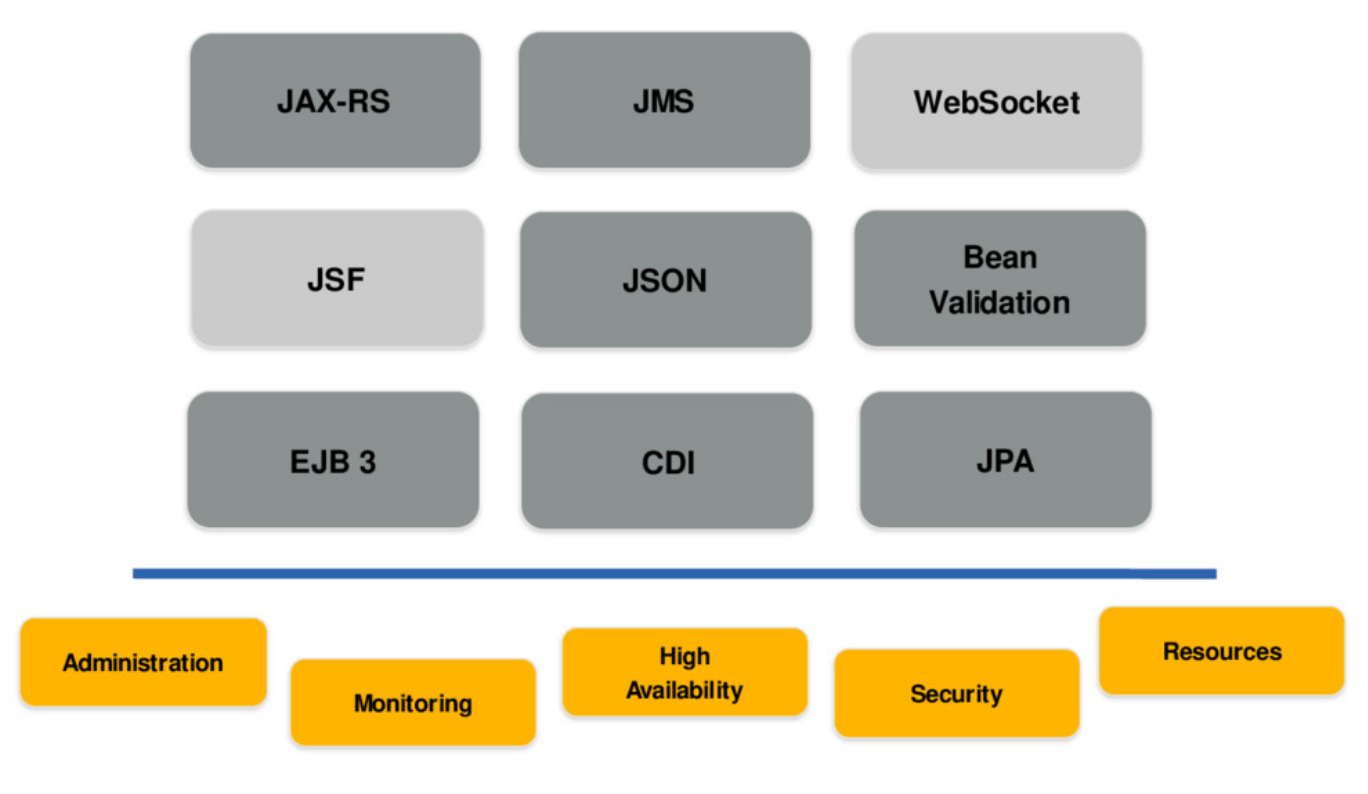
\includegraphics[width=\linewidth]{Images/javaeemicropancake}
    	\caption{Créditos: Reza Rahman}
    \end{figure}

\end{column}
\end{columns}

\end{frame}

\begin{frame}{Microservice Chassis}
\begin{figure}
	\centering
	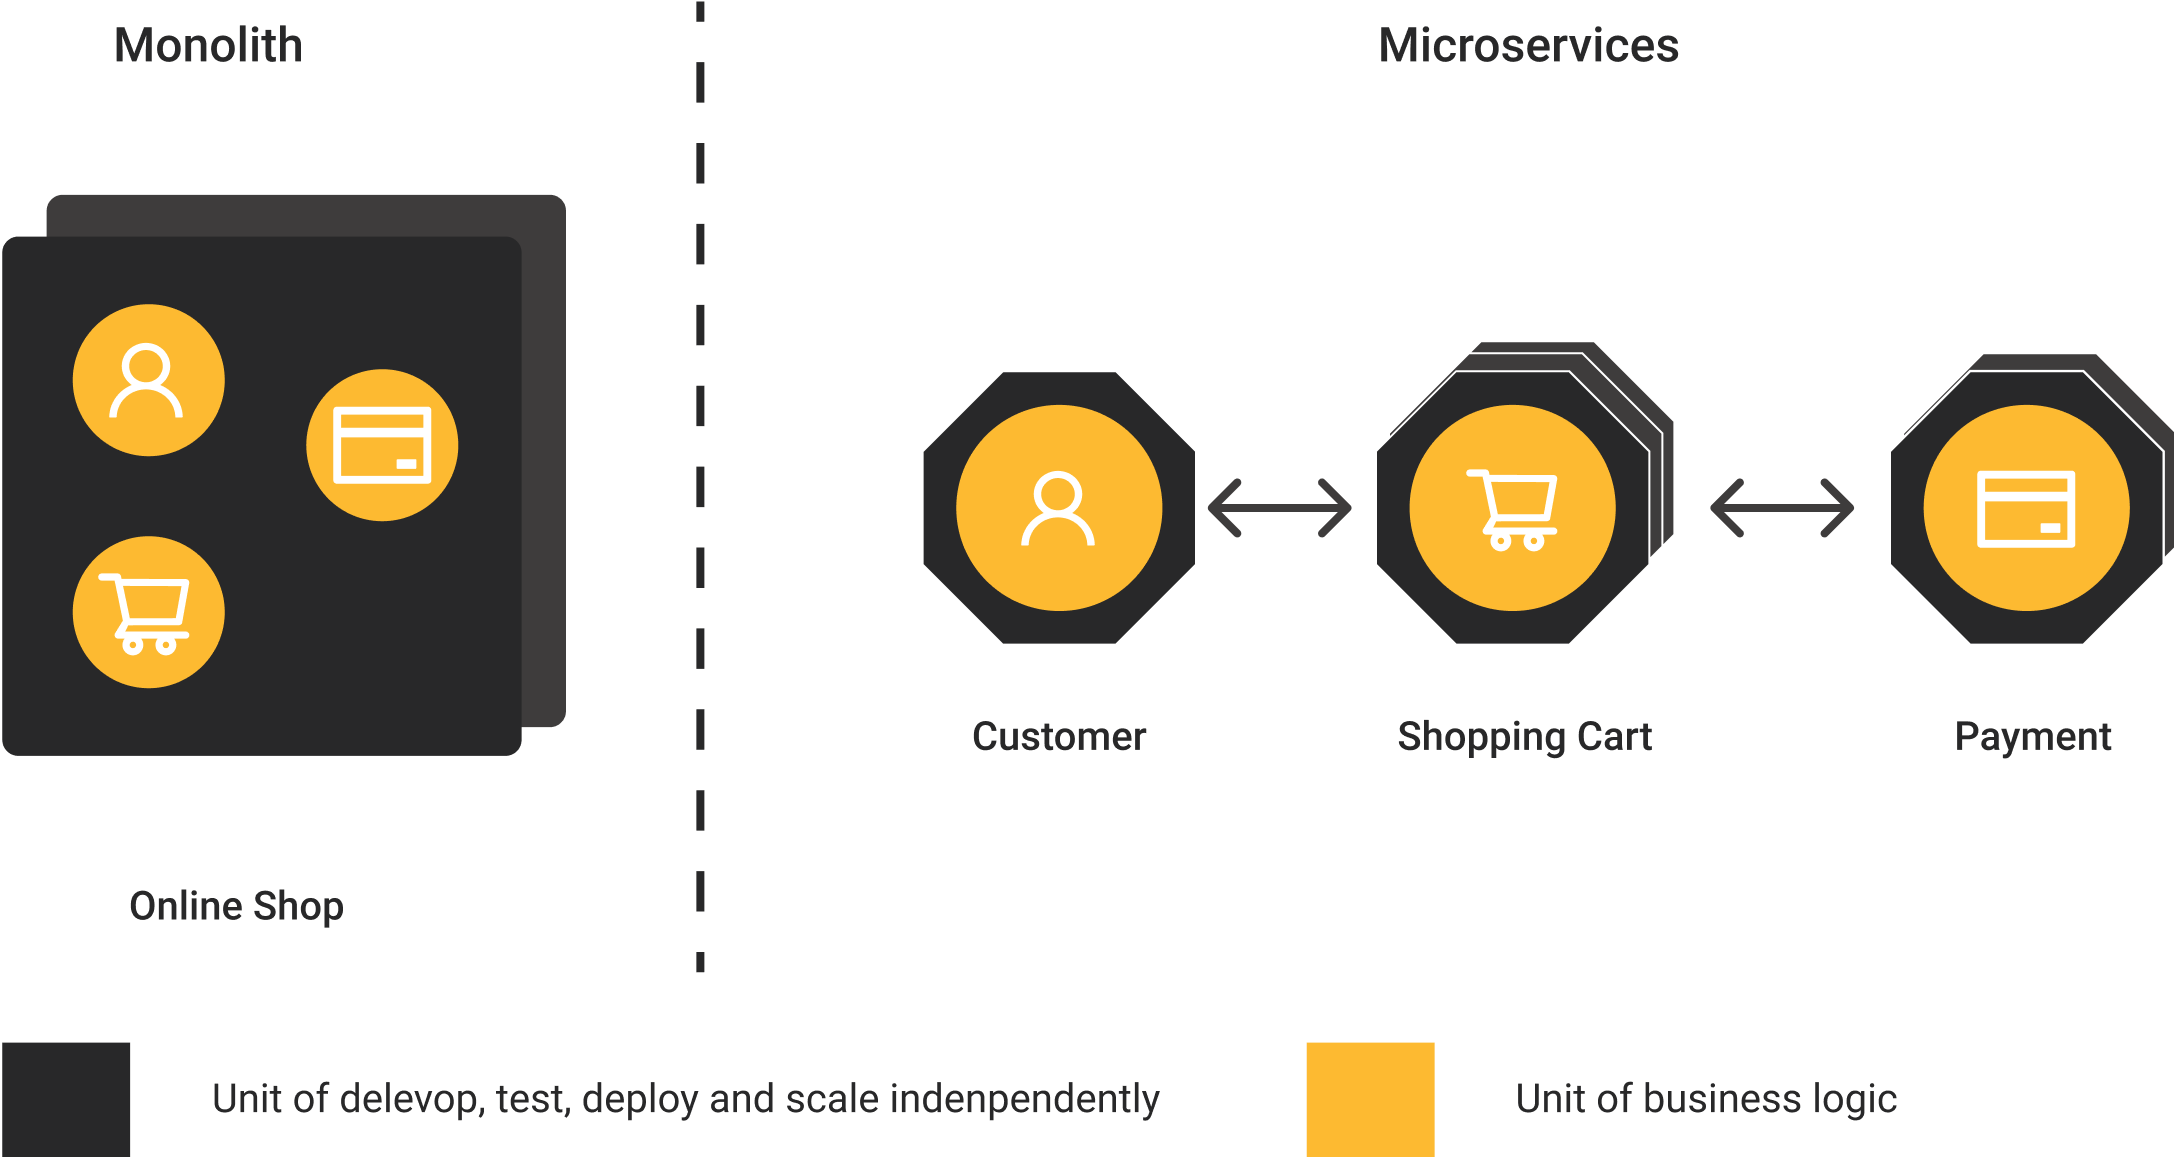
\includegraphics[width=0.7\linewidth]{Images/mp0}
\end{figure}
\end{frame}

\begin{frame}{Coreografia}
Patterns complementarios - Event Sourcing, CQRS
\begin{figure}
	\centering
	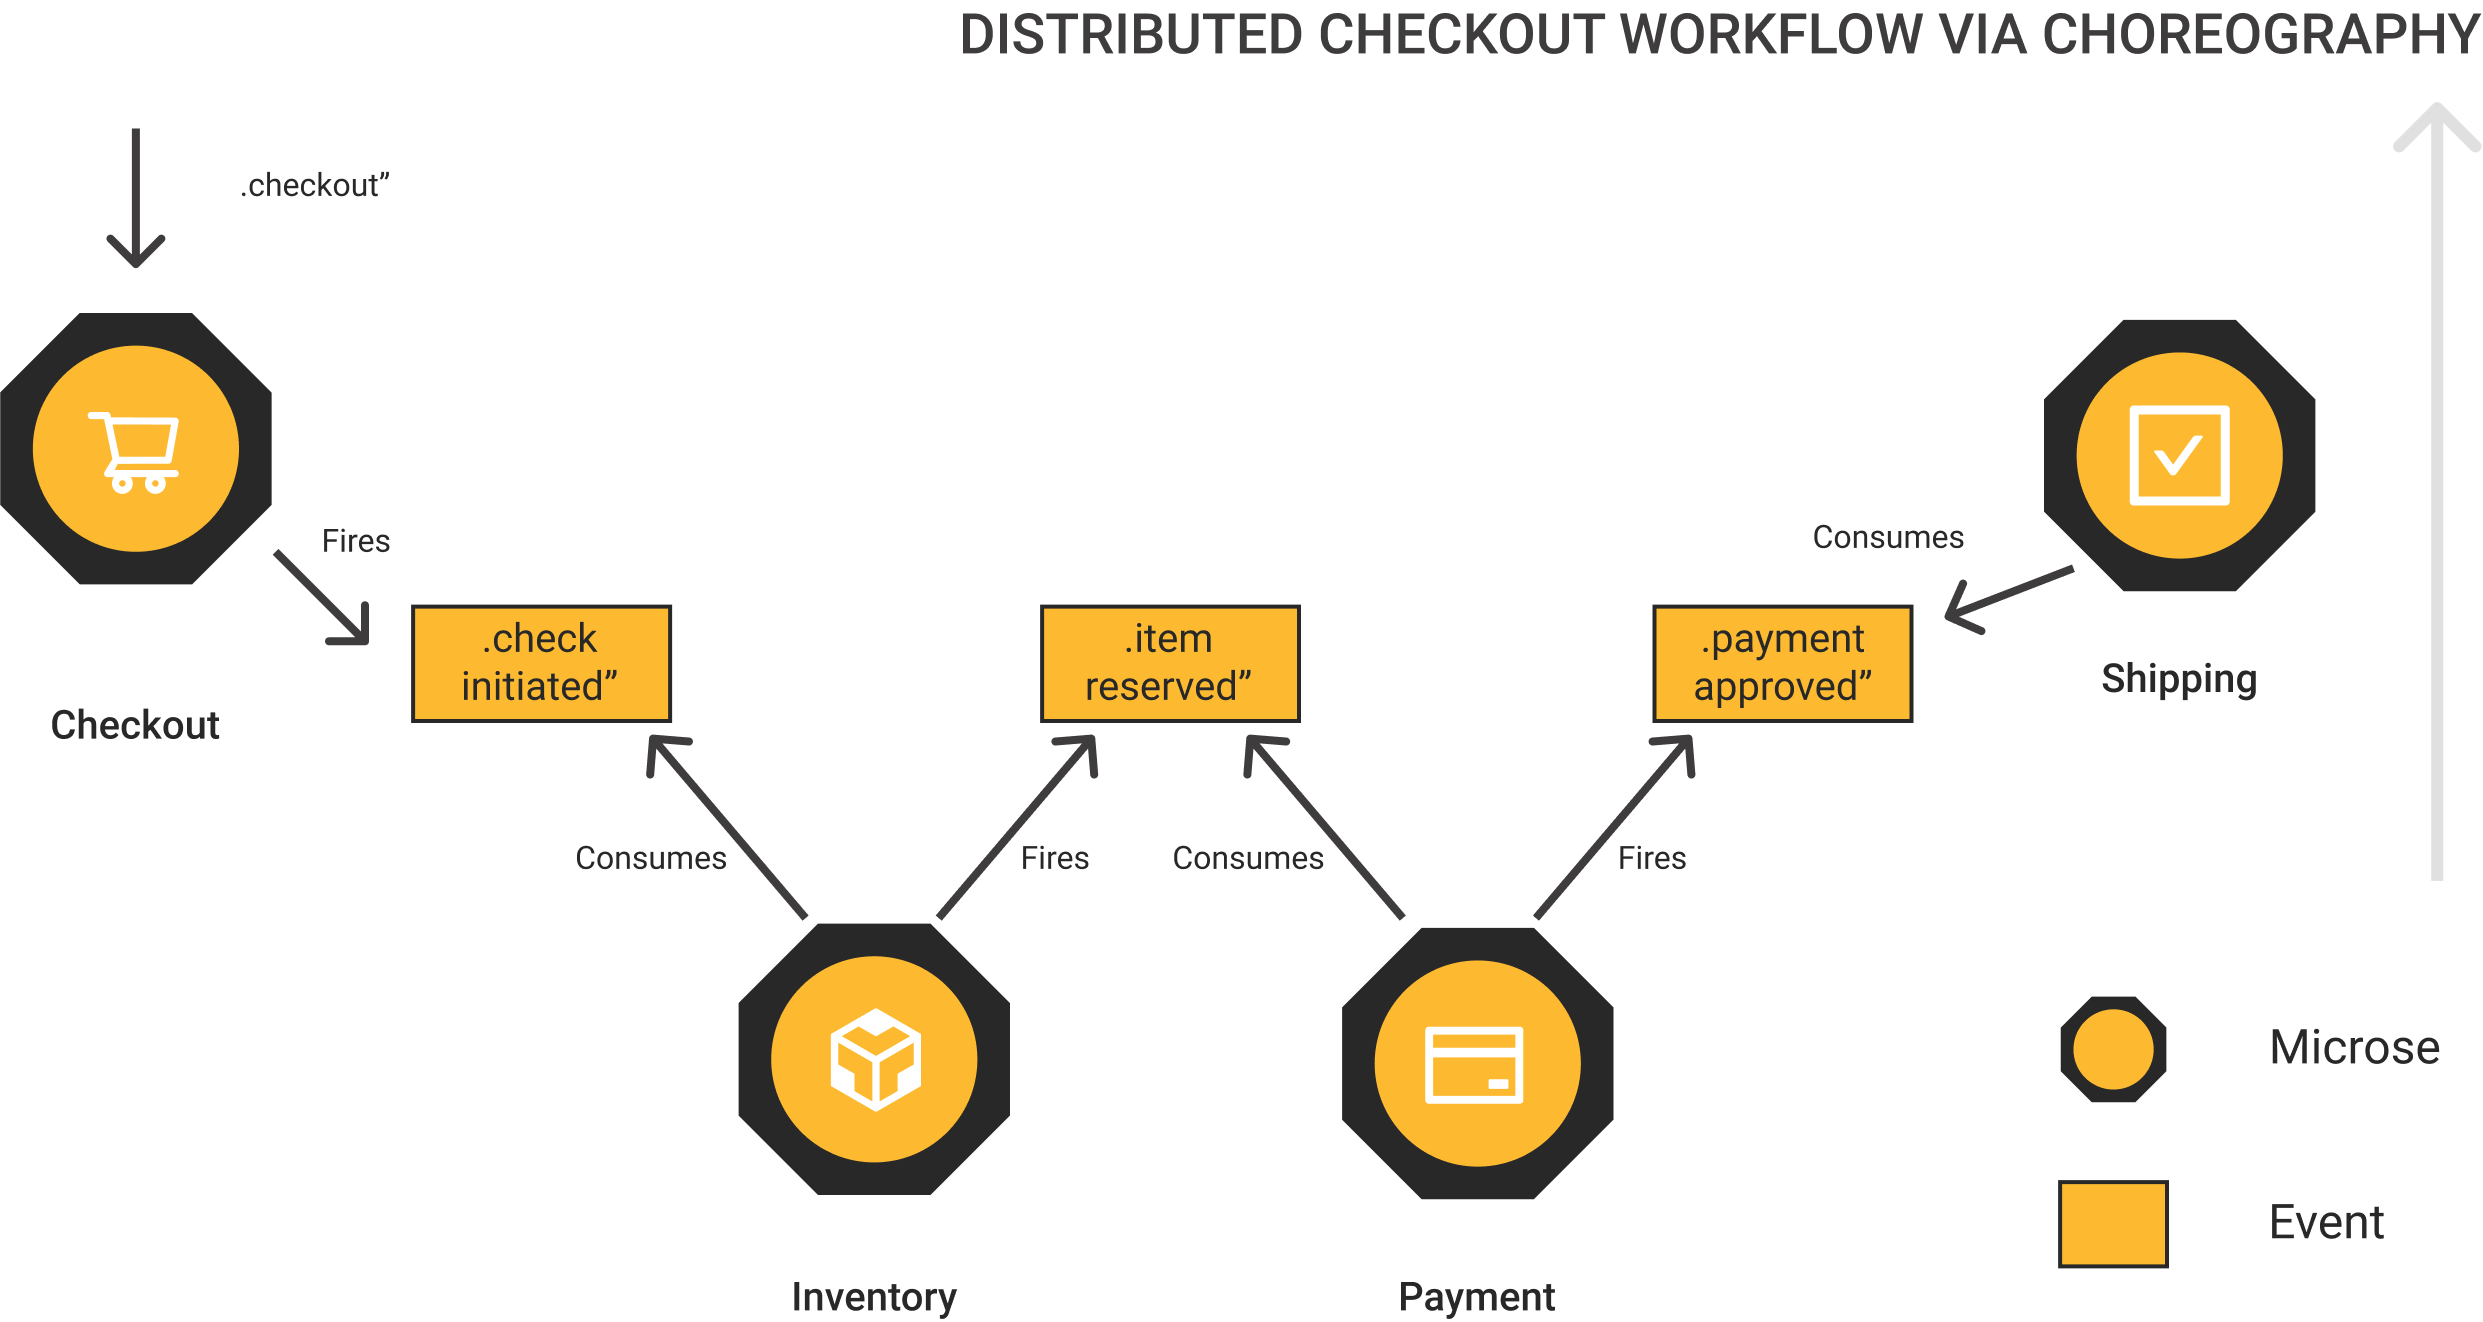
\includegraphics[width=0.7\linewidth]{Images/mpcore}
\end{figure}
\end{frame}

\begin{frame}{Orquestador}
Patterns complementarios - SAGA
\begin{figure}
	\centering
	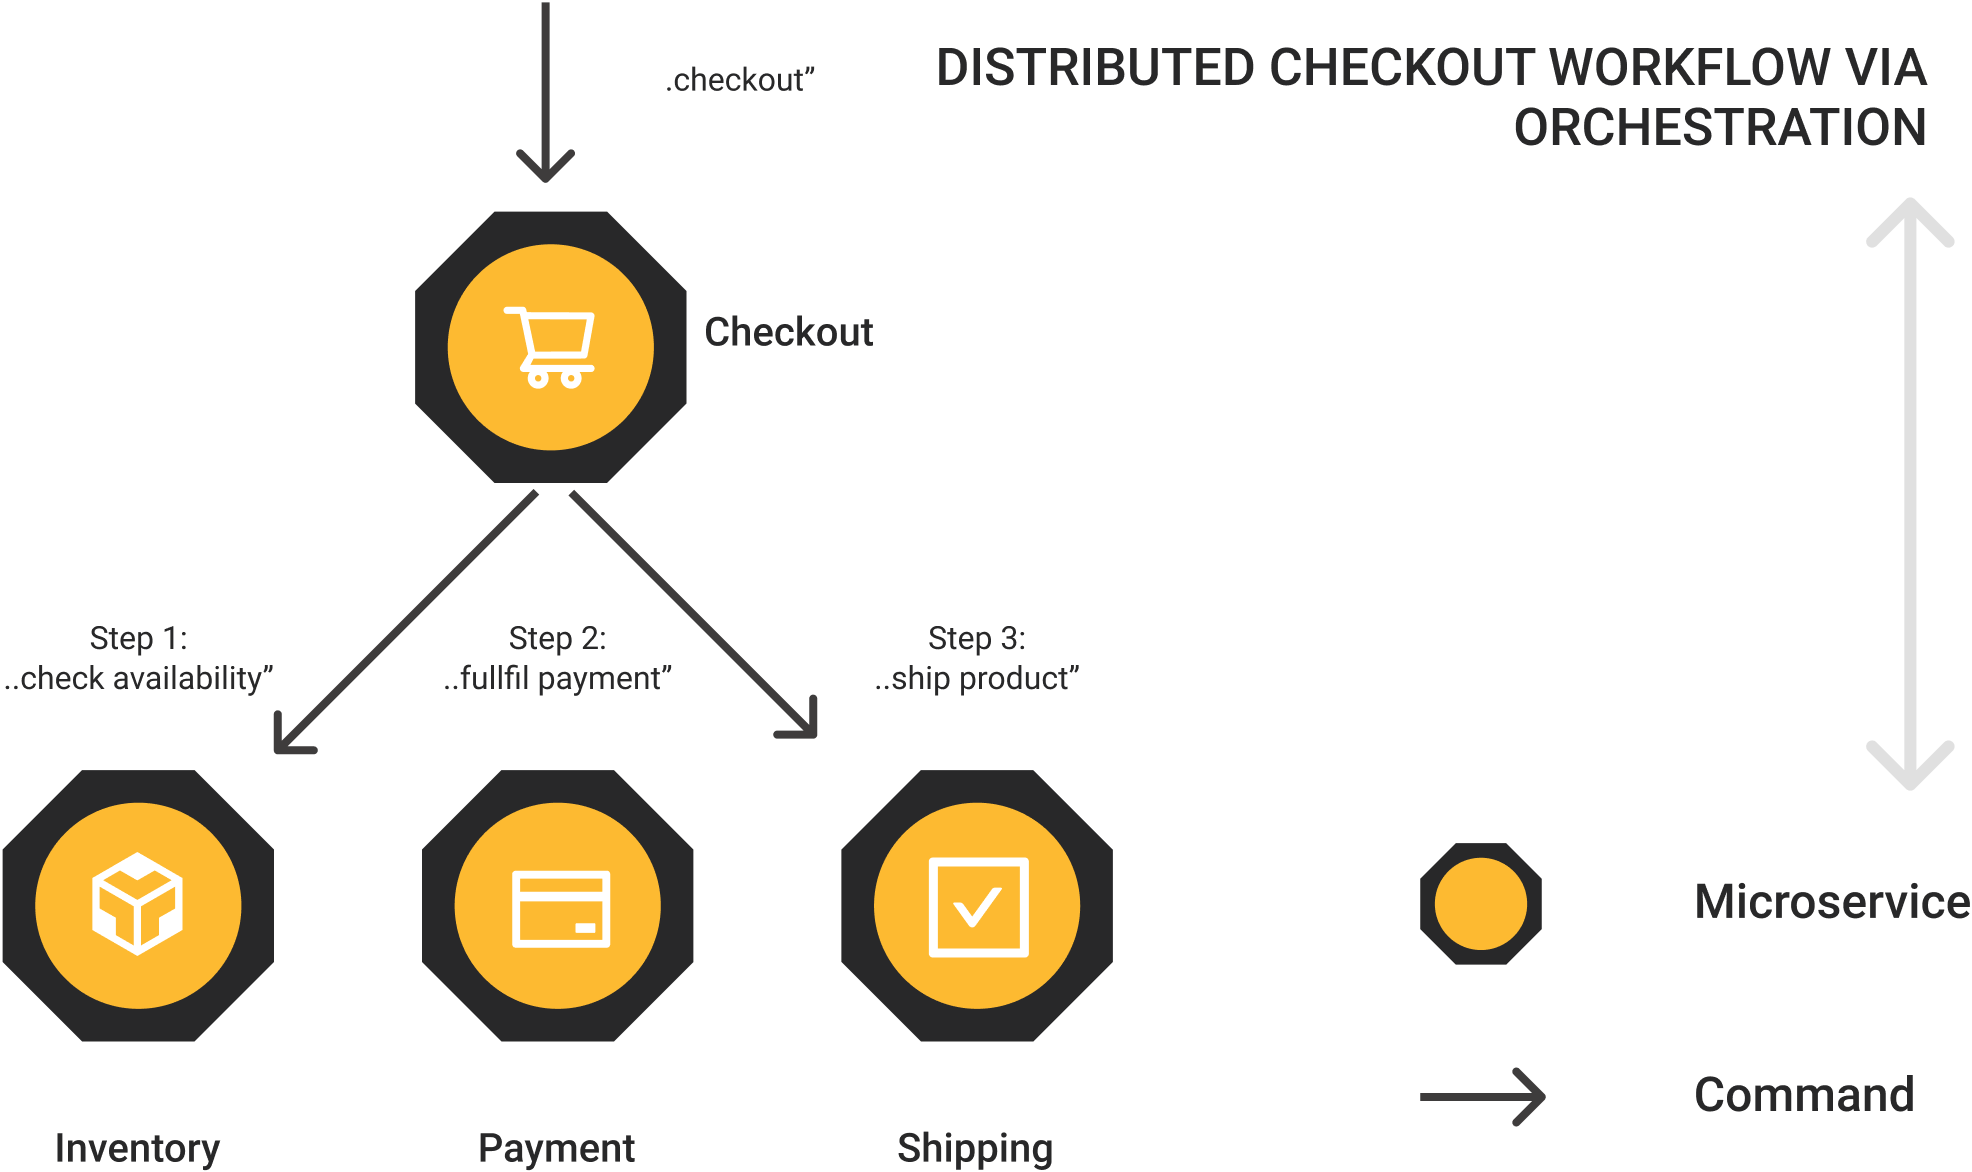
\includegraphics[width=0.7\linewidth]{Images/mporch}
\end{figure}

\end{frame}

\begin{frame}{Cross-cutting en el mundo real}

\begin{itemize}
	\item \textbf{Health checks \& Metrics} - Recolectar métricas  (Prometheus/Grafana) y establecer reglas de despliegue
	\item \textbf{Resilence \& Fault Tolerance} - Service mesh -e.g. Likerd, Istio- y Chassis
	\item \textbf{Configuration} - Inyección de configuración en el ambiente
	\item \textbf{Authentication \& Authorization} - API Gateway + Chassis
	\item \textbf{Standarized documentation} - OpenAPI + Swagger Server
    \item \textbf{Tracing} - Chassis + Zipkin
    \item\textbf{ Remote Procedure \& Messaging} - Chassis + K8S service discovery
\end{itemize}

\end{frame}



\begin{frame}{Víctor Orozco}
    \begin{columns}[T] % contents are top vertically aligned

        \begin{column}[T]{4cm} % alternative top-align that's better for graphics
            \begin{figure}
                \centering
                
\includegraphics[width=\linewidth]{Images/logos}
            \end{figure}
        \end{column}
        \begin{column}[T]{6cm} % each column can also be its own environment
            \begin{itemize}
                \item vorozco@nabenik.com
                \item \href{https://twitter.com/tuxtor}{@tuxtor}
                \item \href{http://vorozco.com}{http://vorozco.com}
                \item \href{http://tuxtor.shekalug.org}{http://tuxtor.shekalug.org}
            \end{itemize}
            \begin{center}
                
\includegraphics[width=0.1\linewidth]{Images/cclogo}
                \\
                This work is licensed under Creative Commons Attribution-NonCommercial-ShareAlike 3.0 Guatemala (CC BY-NC-SA 3.0 GT).
            \end{center}
        \end{column}
    \end{columns}
\end{frame}



\end{document}
